
\documentclass{article}
\usepackage[utf8]{inputenc}
\usepackage[T5]{fontenc}
\usepackage{graphicx}
\usepackage[margin=1.5cm]{geometry}
\title{Lab 6: Map}
\author{Nguyễn Thanh Hùng -- 2540056}
\date{}
\begin{document}
\maketitle
Each 2D thread transforms one grayscale pixel: threshold 128 for binarization, clamped $1.2p+30$ for brightness, or $0.5I_1+0.5I_2$ for blending.
The second image is resized to match the first. Several 2D blocks are timed, and NumPy references validate the saved outputs.

Kernel timing uses \texttt{time.time()} after JIT warm-up and CUDA synchronization,
averaged over three GPU runs. Device allocation and host/device copies are excluded.
CPU measurements are single runs. Speedup is relative to the stated CPU implementation.
Actual measurements appear after running the notebook on Colab; no timings are assumed here.
\IfFileExists{results.tex}{\begin{center}
\resizebox{\linewidth}{!}{
\begin{tabular}{llll}
\hline
block & operation & gpu\_ms & max\_error \\
\hline
(8, 8) & binarized & 0.062863 & 0 \\
(8, 8) & brightness & 0.0594457 & 0 \\
(8, 8) & blended & 0.093619 & 0 \\
(16, 16) & binarized & 0.0465711 & 0 \\
(16, 16) & brightness & 0.05428 & 0 \\
(16, 16) & blended & 0.0584126 & 0 \\
(32, 16) & binarized & 0.0404517 & 0 \\
(32, 16) & brightness & 0.0443459 & 0 \\
(32, 16) & blended & 0.0549952 & 0 \\
(32, 32) & binarized & 0.0649293 & 0 \\
(32, 32) & brightness & 0.0596841 & 0 \\
(32, 32) & blended & 0.0685056 & 0 \\
\hline
\end{tabular}
}
\end{center}}{}
\IfFileExists{performance.png}{\begin{center}\includegraphics[width=.75\linewidth]{performance.png}\end{center}}{}
\IfFileExists{images.png}{\begin{center}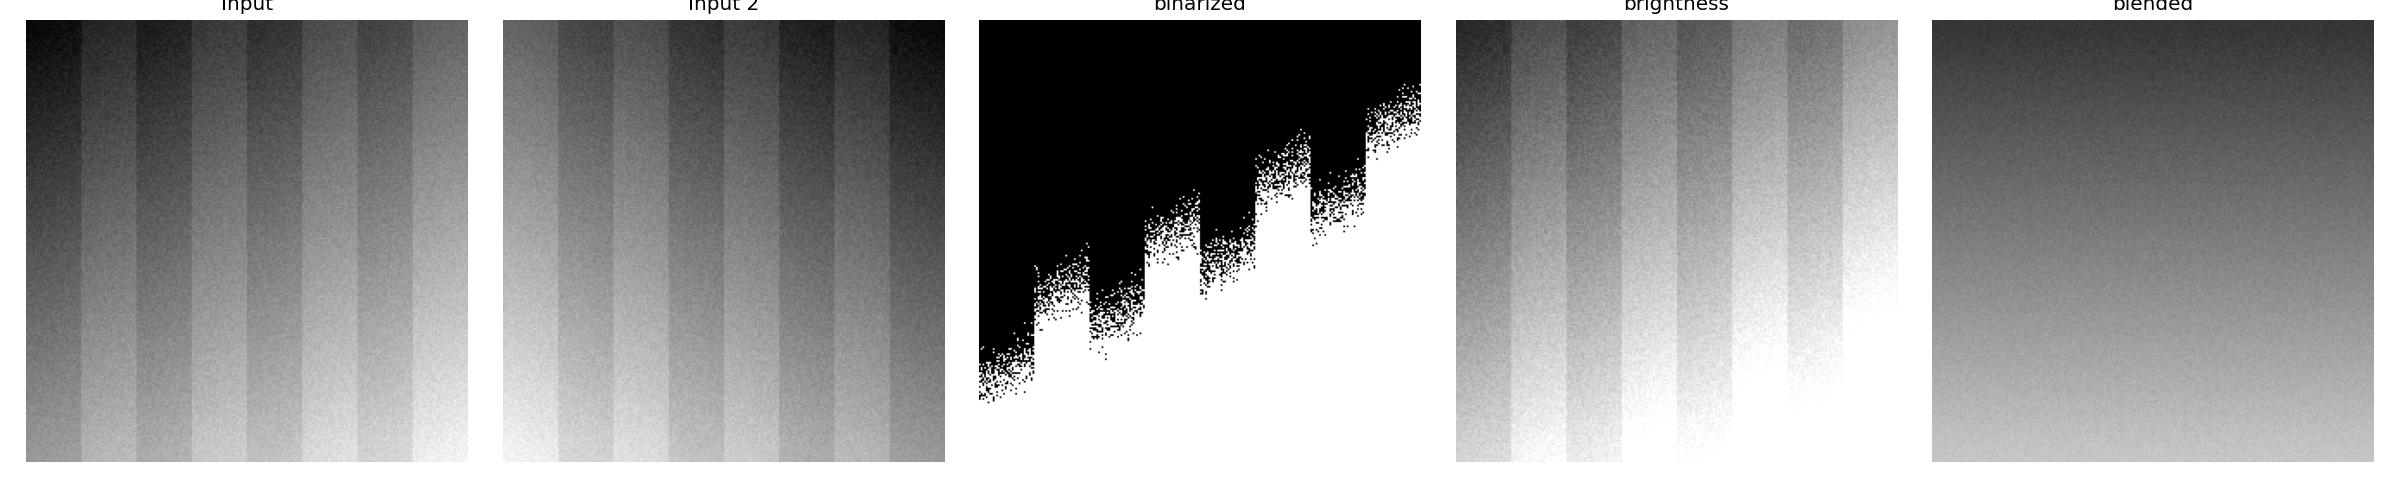
\includegraphics[width=\linewidth]{images.png}\end{center}}{}
\IfFileExists{histograms.png}{\begin{center}\includegraphics[width=.8\linewidth]{histograms.png}\end{center}}{}
\end{document}
